\begin{figure}[h]
  \centering
  \scalebox{0.6}{
  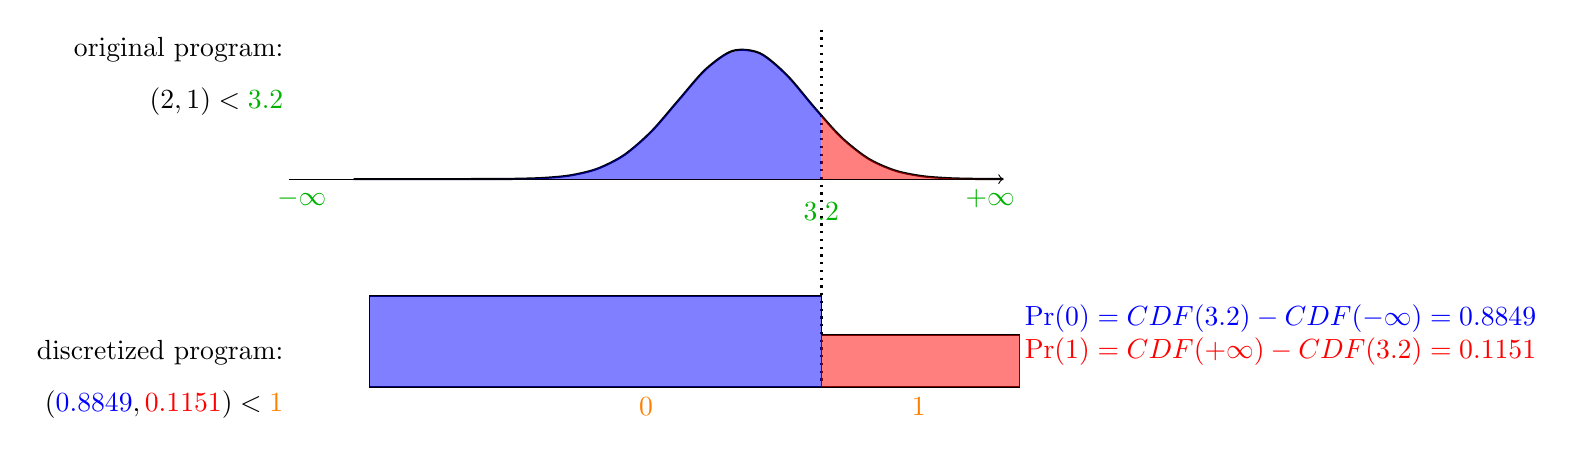
\begin{tikzpicture}[scale=1.1]

  % ===== BEGIN GRAPH REGION =====
  \begin{scope}[xshift=-2.5cm, scale=0.75]

  % Axes for Gaussian
  \draw[->] (-5,0) -- (6,0);
  \node[text=green!70!black] at (-4.8, -0.3) {$-\infty$};
  \node[text=green!70!black] at (5.8, -0.3) {$+\infty$};
  \node[text=green!70!black] at (3.2, -0.5) {3.2};

  % Gaussian curve: N(2,1)
  \draw[thick, domain=-4:6, smooth, variable=\x] 
    plot ({\x},{2*exp(-((\x-2)*(\x-2))/2)});

  % Vertical dotted line 
  \draw[dotted, thick] (3.2, 2.3) -- (3.2, -3.2);

  % Blue shading (left interval)
  \fill[blue, opacity=0.5] 
    (-4,0) -- plot[domain=-4:3.2] (\x,{2*exp(-((\x-2)*(\x-2))/2)}) -- (3.2,0) -- cycle;

  % Red shading (right interval)
  \fill[red, opacity=0.5] 
    (3.2,0) -- plot[domain=3.2:6] (\x,{2*exp(-((\x-2)*(\x-2))/2)}) -- (6,0) -- cycle;

  % Discrete distribution: 0 bar
  \draw (-3.75,-1.8) rectangle (3.2,-3.2);

  % Discrete distribution: 1 bar
  \draw (3.2,-2.4) rectangle (6.25,-3.2);

  % Fill colors
  \fill[blue, opacity=0.5] (-3.75,-1.8) rectangle (3.2,-3.2);
  \fill[red, opacity=0.5] (3.2,-2.4) rectangle (6.25,-3.2);

  % Labels
  \node[text=orange] at (0.5,-3.5) {0};
  \node[text=orange] at (4.7,-3.5) {1};

  \end{scope}
  % ===== END GRAPH REGION =====

  % Original program text
  \node[left] at (-6.2,1.5) {original program:};
  \node[left] at (-6.2,0.9) {$\gaussian(2,1) < \textcolor{green!70!black}{3.2}$};

  % Discretized program text
  \node[left] at (-6.2,-2.0) {discretized program:};
  \node[left] at (-6.2,-2.6) {$\discrete(\textcolor{blue}{0.8849}, \textcolor{red}{0.1151}) < \textcolor{orange}{1}$};

  % Probability equations
  \node[align=left] at (5.2,-1.8) {
  \textcolor{blue}{$\Pr(0) = CDF(3.2) - CDF(-\infty)= 0.8849$}\\
  \textcolor{red}{$\Pr(1) = CDF(+\infty) - CDF(3.2) = 0.1151$}
  };

  \end{tikzpicture}
  }
  \caption{Discretization of the original program $\gaussian(2,1) < 3.2$ into the semantically equivalent discretized program $\discrete(0.8849, 0.1151) < 1$. The blue and red shaded regions show how the cut at 3.2 partitions the continuous distribution into two intervals $(-\infty, 3.2)$ and $[3.2, +\infty)$, whose masses become the probabilities of outcomes $0$ and $1$, e.g. interval indices, in the discrete distribution.}
  \label{fig:cuts-gaussian}
\end{figure}

\iffalse
\begin{figure}
    \centering
    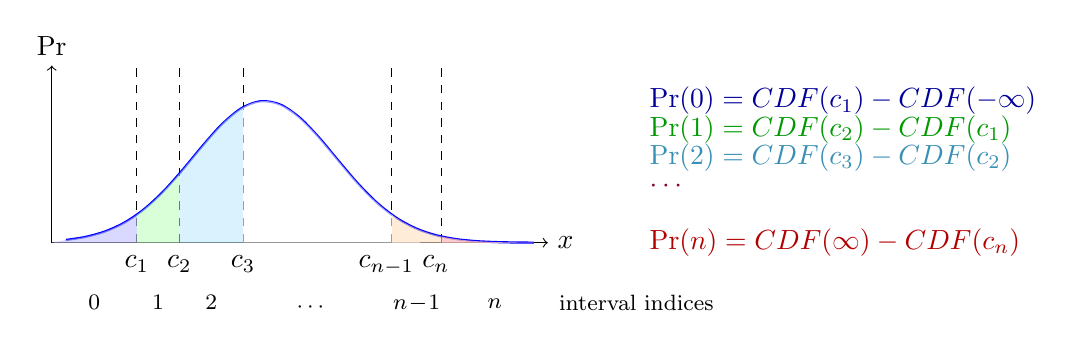
\begin{tikzpicture}[scale=0.9]
      % Axes
      \draw[->] (0,0) -- (7,0) node[right] {$x$};
      \draw[->] (0,0) -- (0,2.5) node[above] {$\Pr$};
    
      % Continuous distribution curve
      \draw[domain=0.2:6.8, smooth, variable=\x, thick, blue]
        plot ({\x}, {2*exp(-0.5*((\x-3)^2))});
    
      % Vertical cut lines with labels (shift c_{n-1} and c_n left slightly)
      \foreach \x/\label in {1.2/$c_1$, 1.8/$c_2$, 2.7/$c_3$, 4.8/{\hspace{-4pt}$c_{n-1}$}, 5.5/{\hspace{-4pt}$c_n$}} {
        \draw[dashed] (\x,0) -- (\x,2.5);
        \node[below] at (\x,-0.05) {\label};
    }
    
      % Shading intervals (different colors)
      \fill[blue!25, opacity=0.6] (0,0)
          -- plot[domain=0.2:1.2] ({\x}, {2*exp(-0.5*((\x-3)^2))})
          -- (1.2,0) -- cycle;
    \fill[green!25, opacity=0.6] (1.2,0)
          -- plot[domain=1.2:1.8] ({\x}, {2*exp(-0.5*((\x-3)^2))})
          -- (1.8,0) -- cycle;
      \fill[cyan!25, opacity=0.6] (1.8,0)
          -- plot[domain=1.8:2.7] ({\x}, {2*exp(-0.5*((\x-3)^2))})
          -- (2.7,0) -- cycle;
      \fill[white!25, opacity=0.6] (2.7,0)
          -- plot[domain=2.7:4.8] ({\x}, {2*exp(-0.5*((\x-3)^2))})
          -- (5.2,0) -- cycle;
      \fill[orange!25, opacity=0.6] (4.8,0)
            -- plot[domain=4.8:5.5] ({\x},{2*exp(-0.5*((\x-3)^2))})
            -- (5.5,0) -- cycle;
      \fill[red!25, opacity=0.8] (5.5,0)
            -- plot[domain=5.5:6.8] ({\x},{2*exp(-0.5*((\x-3)^2))})
            -- (6.8,0) -- cycle;

    % Interval number labels (shift n-1 and n left slightly)
    \node[below] at (0.6,-0.6) {\footnotesize $0$};
    \node[below] at (1.5,-0.6) {\footnotesize$1$};
    \node[below] at (2.25,-0.6) {\footnotesize$2$};
    \node[below] at (3.65,-0.7) {\footnotesize$\cdots$};
    \node[below] at (5.15,-0.6) {\footnotesize$n\!-\!1$};   % shifted 0.1 left
    \node[below] at (6.25,-0.65) {\footnotesize$n$};         % shifted 0.15 left
       \node[below] at (8.25,-0.6) {\footnotesize interval indices}; 
      % Color-matched probability annotations
      \node[right, text=blue!60!black]  at (8.3,2.0) {$\Pr(0) = \text{CDF}(c_1) - \text{CDF}(-\infty)$};
      \node[right, text=green!60!black]   at (8.3,1.6) {$\Pr(1) = \text{CDF}(c_2) - \text{CDF}(c_1)$};
      \node[right, text=cyan!70!black]at (8.3,1.2) {$\Pr(2) = \text{CDF}(c_3) - \text{CDF}(c_2)$};
      \node[right, text=purple!70!black]at (8.3,0.8) {$\cdots$};
      \node[right, text=red!70!black]   at (8.3,0.0) {$\Pr(n) = \text{CDF}(\infty) - \text{CDF}(c_n)$};
    
    \end{tikzpicture}
    \caption{Partitioning a continuous distribution by cuts $\clt{c_1}, \ldots, \clt{c_n}$ into intervals $(-\infty, c_1), [c_1,c_2), \ldots, [c_n, +\infty)$, with each interval assigned a discrete probability $\Pr(i)$ computed from CDF differences. Each interval represents a range of real values that is abstracted to a single discretized value labeled $0, 1, \ldots, n$. Note the resulting intervals may vary in width and need not be uniformly spaced. Given an expression of type $\floattype{B}{V}$, a finite value set $V$ maps the expression to the unique interval containing that value, whereas $V = \top$ yields a discrete distribution over all interval indices $i$, weighted by their probabilities $\Pr(i)$.}
    \label{fig:cuts-distr}
\end{figure}
\fi